% =====================================================================
% A Simulation-Based Reproduction of Comparative Sensor Fusion
% Algorithms for a Miniature IMU --- Sansone, Bartolini, Perin, Badia
% (ISITIA 2023) Reproduced on Synthetic MPU-6050 Data with an
% Analytical ATmega328P Timing Model
%
% Authors: Abdullah Altepe, Mehmet Bahceci, Yusuf Oruc, Murat Demir
% Marmara University, Department of Electrical and Electronics Engineering
%
% Compile with pdflatex (Overleaf works out of the box).
% =====================================================================

\documentclass[conference]{IEEEtran}
\IEEEoverridecommandlockouts

\usepackage{cite}
\usepackage{amsmath,amssymb,amsfonts}
\usepackage{graphicx}
\usepackage{textcomp}
\usepackage{xcolor}
\usepackage{booktabs}
\usepackage{array}
\usepackage{tikz}
\usetikzlibrary{shapes.geometric,arrows.meta,positioning,calc,fit}
\usepackage{url}
\usepackage[hidelinks]{hyperref}

% --- a few convenience macros ---
\newcommand{\bm}[1]{\mathbf{#1}}
\newcommand{\R}{\mathbb{R}}
\newcommand{\unit}[1]{\,\mathrm{#1}}
\newcommand{\degr}{^{\circ}}

\begin{document}

\title{A Simulation-Based Reproduction of Comparative Sensor
Fusion Algorithms on a Miniature IMU\\
{\large Replicating Badia \textit{et al.} (ISITIA 2023) with a
Synthetic MPU-6050 Data Pipeline and an Analytical ATmega328P
Timing Model}}

\author{
\IEEEauthorblockN{Abdullah Altepe, Mehmet Bah\c{c}eci, Yusuf Oru\c{c}, Murat Demir}
\IEEEauthorblockA{Department of Electrical and Electronics Engineering\\
Marmara University, Istanbul, T\"urkiye\\
\{abdullah.altepe, mehmet.bahceci, yusuf.oruc, murat.demir\}@marun.edu.tr}
}

\maketitle

% =====================================================================
\begin{abstract}
Estimating the orientation of a rigid body from a low-cost inertial
measurement unit (IMU) is a recurring problem in drones, wearables,
self-balancing robots, virtual reality headsets and educational
robotics. Sansone, Bartolini, Perin and Badia (ISITIA 2023) compared
four candidate orientation-estimation methods --- direct
trigonometric computation, a one-dimensional Kalman filter, the
Madgwick gradient-descent filter, and the Mahony complementary
filter --- on an InvenSense MPU-6050 connected to an Arduino Nano,
and concluded that the Kalman filter is the most accurate, the
Mahony filter is the cheapest per integration step, and the
Madgwick filter sits in between. This paper presents a
\emph{simulation-based reproduction} of that comparison. All four
algorithms are independently re-implemented in Python; the
accuracy comparison is run on synthetic MPU-6050 measurements
generated from a known ground-truth tilt trajectory with realistic
sensor noise and bias; the per-step computation cost on the
ATmega328P is estimated analytically from a published
floating-point cycle-cost model. Three of the four qualitative
claims of the reference paper are confirmed on our pipeline (Mahony
fastest among the filters, Madgwick and Kalman nearly equal in
compute, Kalman dominates noise rejection together with Mahony at
$k_p=10$); one diverges (in our analytical timing model the
trigonometric estimator is the cheapest method, not the most
expensive). Code, data and the LaTeX source of this paper are
released publicly so that an independent third group can repeat
both Badia \textit{et al.} and our reproduction.
\end{abstract}

\begin{IEEEkeywords}
Sensor fusion, inertial measurement unit, MPU-6050, Arduino Nano,
Kalman filter, Madgwick filter, Mahony filter, orientation
estimation, reproducibility, simulation.
\end{IEEEkeywords}

% =====================================================================
\section{Introduction}\label{sec:intro}

Knowing how an object is oriented in three-dimensional space is one
of those deceptively simple problems that keeps reappearing across
modern engineering. A drone needs an attitude estimate to stay level
in the air, a self-balancing robot needs it to remain upright, a VR
headset needs it to keep the virtual world steady on the user's
face, and a wearable activity tracker needs it to decide whether
the wrist is walking or merely waving. In all of these cases the
underlying measurement comes from the same family of sensors: a
small, inexpensive, MEMS-based inertial measurement unit (IMU)
that integrates a tri-axis accelerometer and a tri-axis gyroscope
into a single die.

The fundamental difficulty is that neither sensor, taken alone, is
sufficient. A gyroscope reports angular velocity directly and is
smooth and responsive over short time windows, but converting
angular velocity into an absolute orientation requires temporal
integration, and even a small constant bias produces an angular
error that grows linearly with time. An accelerometer reports the
specific force on the body; when the body is nearly static, that
specific force is dominated by gravity, so roll and pitch can be
recovered directly without integration and without long-term
drift, but the signal is noisy and is corrupted by every vibration
or jolt. The gyroscope is \emph{smooth but drifts}, the
accelerometer is \emph{stable but noisy}; combining them produces
an estimate that is better than either source alone. This is the
elementary motivation for sensor fusion in attitude estimation.

The setting becomes considerably tighter when the platform is
itself low-cost. Sansone, Bartolini, Perin and Badia,
in their ISITIA 2023 paper~\cite{badia2023}, place exactly this
question on an InvenSense MPU-6050 wired over $\mathrm{I}^2\mathrm{C}$ to an Arduino
Nano --- an 8-bit ATmega328P microcontroller with $2\,\mathrm{kB}$
of SRAM and a $16\,\mathrm{MHz}$ clock. On that kind of hardware,
elegance on paper is not enough; the filter must run in real time
with budget to spare. The authors compare four reasonable choices
for the orientation estimator --- a direct trigonometric
computation, a one-dimensional Kalman filter, the Madgwick
gradient-descent filter, and the Mahony complementary filter ---
and report a clear tradeoff between accuracy and per-step
computation time.

The work reported here is a \emph{simulation-based} reproduction
of Badia \textit{et al.}~\cite{badia2023}. Hardware was not
available to the authors at the time of writing; in its place we
use (i) a fully controlled synthetic IMU data pipeline that mimics
the MPU-6050 noise and bias characteristics, and (ii) an
analytical floating-point cycle-cost model of the ATmega328P that
allows per-step computation time to be estimated directly from
operation counts in the source code. This simulation-based path
trades a little realism on the noise side for two unique
advantages: the ground-truth orientation is exact rather than
mechanically estimated, and the entire experiment is bit-for-bit
reproducible by anyone willing to re-run the released code.

The contribution of this paper is therefore not a new algorithm.
It is (i) a complete, independent re-implementation of the four
algorithms compared by Badia \textit{et al.}; (ii) a quantitative
test of the four numerical claims of the reference paper on a
controlled synthetic dataset; (iii) an analytical timing model for
ATmega328P float operations that lets the per-step compute
ranking be obtained without an Arduino board in hand; and
(iv) a publicly released code base~\cite{ourcode} that any third
group can use to repeat both the original paper and our
reproduction.

The remainder of the paper is structured as follows.
Section~\ref{sec:refpaper} summarises the reference paper and
states the precise numerical claims that we test.
Section~\ref{sec:math} develops the mathematical background for the
four algorithms with enough detail to allow a clean
re-implementation.
Section~\ref{sec:setup} documents the synthetic data pipeline and
the analytical timing model that together replace the physical
testbed.
Section~\ref{sec:protocol} is the experimental protocol:
parameter lock-ins, the static-tilt scenario, the timing
methodology, the reported metrics, and the success criterion.
Section~\ref{sec:results} reports the measured numbers and the
figures that come with them.
Section~\ref{sec:disc} discusses the one divergence we observe
from the reference paper.
Section~\ref{sec:threats} lists the threats to validity and
Section~\ref{sec:conclusion} concludes.

% =====================================================================
\section{The Reference Paper and Reproduction Targets}\label{sec:refpaper}

\subsection{What Badia \textit{et al.} Did}

The reference paper~\cite{badia2023} targets ``miniature IMU
measurements,'' by which the authors mean the kind of low-cost
MEMS IMU that appears in Tactile-Internet devices, hobby drones,
consumer wearables, and educational robotics. The hardware used is
an InvenSense MPU-6050 (tri-axis accelerometer at $\pm 2\,g$
default, tri-axis gyroscope at $\pm 250\degr/\mathrm{s}$ default)
connected over $\mathrm{I}^2\mathrm{C}$ to an Arduino Nano based on
the ATmega328P microcontroller. The four orientation-estimation
methods are implemented directly on the microcontroller:
\begin{enumerate}
\item \textbf{Trigonometric computation.} Roll and pitch are
recovered from the accelerometer vector via \texttt{atan2}, with
no fusion and no filtering.
\item \textbf{Kalman filter.} A one-dimensional Kalman filter
fuses the integrated gyroscope rate with the accelerometer-derived
angle through explicit process and measurement noise covariances.
\item \textbf{Madgwick filter.} A gradient-descent quaternion
filter with a single tuning parameter $\beta$.
\item \textbf{Mahony filter.} A complementary-style quaternion
filter that uses a proportional--integral correction driven by the
cross product between the measured and the predicted gravity
direction.
\end{enumerate}
For each of these the authors record roll/pitch estimates around
reference static tilts (approximately $\pm 15\degr$) and measure
per-integration-step computation time directly on the
microcontroller.

\subsection{The Numerical Claims We Reproduce}

The reference paper's main quantitative conclusions, which this
project tests on its synthetic pipeline, are:
\begin{itemize}
\item C1. The trigonometric method is the most exposed to
accelerometer noise.
\item C2. The Kalman filter and the Madgwick filter take comparable
amounts of time per integration step, with the Kalman filter
producing the most stable estimate.
\item C3. The Mahony filter is the fastest per-step filter on the
target microcontroller, at a small cost in accuracy.
\item C4. If accuracy is the design priority, the Kalman filter is
preferred; if compute is tight, the Mahony filter is preferred;
the Madgwick filter occupies an intermediate point in the
tradeoff.
\end{itemize}
We also test, as a fifth implicit claim, the ranking of the
trigonometric method on the compute axis (the reference paper
reports it as the most expensive of the four), and report a
divergence below.

% =====================================================================
\section{Mathematical Background}\label{sec:math}

\subsection{Notation, Frames, and Sensor Models}

Let $\{B\}$ denote the body frame fixed to the IMU and $\{W\}$
denote a world frame whose $z$ axis is aligned with the local
gravity vector $\bm{g} = [0,0,g]^\top$ with $g \approx
9.81\,\mathrm{m}/\mathrm{s}^2$. Orientation is described either by
the Euler triplet $(\phi,\theta,\psi)$ for roll, pitch and yaw, or
by a unit quaternion $\bm{q} = [q_0,q_1,q_2,q_3]^\top$ with
$\|\bm{q}\| = 1$. The associated rotation matrix is
\begin{equation}
\bm{R}(\bm{q}) =
\begin{bmatrix}
q_0^2+q_1^2-q_2^2-q_3^2 & 2(q_1q_2-q_0q_3) & 2(q_1q_3+q_0q_2)\\
2(q_1q_2+q_0q_3) & q_0^2-q_1^2+q_2^2-q_3^2 & 2(q_2q_3-q_0q_1)\\
2(q_1q_3-q_0q_2) & 2(q_2q_3+q_0q_1) & q_0^2-q_1^2-q_2^2+q_3^2
\end{bmatrix}.
\end{equation}

The simplified accelerometer and gyroscope measurement models are
\begin{align}
\bm{a}_m &= \bm{R}(\bm{q})^\top \bm{g} + \bm{b}_a + \bm{n}_a, \\
\boldsymbol{\omega}_m &= \boldsymbol{\omega} + \bm{b}_g + \bm{n}_g,
\end{align}
where $\bm{n}_a$ and $\bm{n}_g$ are zero-mean white Gaussian noise
processes and $\bm{b}_a$, $\bm{b}_g$ are slowly-varying
accelerometer and gyroscope biases.

\subsection{Trigonometric Computation}

The most direct estimator simply inverts the static-equilibrium
accelerometer model algebraically. Writing the accelerometer
reading as $(a_x,a_y,a_z)$, roll and pitch are recovered by
\begin{align}
\phi &= \mathrm{atan2}\bigl(a_y,\, a_z\bigr), \\
\theta &= \mathrm{atan2}\bigl(-a_x,\, \sqrt{a_y^2 + a_z^2}\bigr).
\end{align}
This estimator has zero long-term drift but reproduces every bit
of accelerometer noise unfiltered into the angle estimate, and it
is undefined for yaw. It serves as the unfused baseline.

\subsection{Kalman Filter (1D / 2D Euler Form)}

For each axis (roll and pitch), the reference paper uses a
two-state linear Kalman filter whose state contains the angle
$\theta_k$ and the gyroscope bias $b_k$:
\begin{equation}
\bm{x}_k =
\begin{bmatrix}\theta_k\\ b_k\end{bmatrix},\quad
\bm{F} =
\begin{bmatrix}1 & -\Delta t \\ 0 & 1\end{bmatrix},\quad
\bm{B} =
\begin{bmatrix}\Delta t \\ 0\end{bmatrix},\quad
\bm{H} = \begin{bmatrix}1 & 0\end{bmatrix}.
\end{equation}
The control input is the measured gyroscope rate $\omega_k$ on
that axis, the measurement is the accelerometer-derived angle
$\theta_k^{\mathrm{acc}}$ obtained by the previous formulas. The
predict / update equations are the standard ones,
\begin{align}
\hat{\bm{x}}_{k|k-1} &= \bm{F}\hat{\bm{x}}_{k-1|k-1} + \bm{B}\omega_{k-1},\\
\bm{P}_{k|k-1} &= \bm{F}\bm{P}_{k-1|k-1}\bm{F}^\top + \bm{Q},\\
\bm{K}_k &= \bm{P}_{k|k-1}\bm{H}^\top
\bigl(\bm{H}\bm{P}_{k|k-1}\bm{H}^\top + R\bigr)^{-1},\\
\hat{\bm{x}}_{k|k} &= \hat{\bm{x}}_{k|k-1}
+ \bm{K}_k\bigl(\theta_k^{\mathrm{acc}} - \bm{H}\hat{\bm{x}}_{k|k-1}\bigr),\\
\bm{P}_{k|k} &= (\bm{I} - \bm{K}_k\bm{H})\bm{P}_{k|k-1}.
\end{align}
The two filters (one for roll, one for pitch) run in parallel and
together provide the two-degree-of-freedom estimate that the
reference paper compares. Yaw is not estimated; the MPU-6050 has
no magnetometer.

\subsection{Madgwick Filter}

Madgwick~\cite{madgwick2010} formulates orientation estimation as
the minimisation of an error function comparing the predicted
gravity direction with the normalised accelerometer reading,
\begin{equation}
\bm{f}(\bm{q},\hat{\bm{a}}) = \bm{R}(\bm{q})^\top \hat{\bm{g}} - \hat{\bm{a}},
\end{equation}
where $\hat{\bm{g}} = [0,0,1]^\top$. A single gradient-descent
step is taken per sample and combined with the integrated
gyroscope rate $\dot{\bm{q}}_{\mathrm{gyro}} = \tfrac{1}{2}
\bm{q} \otimes [0,\boldsymbol{\omega}_m^\top]^\top$:
\begin{equation}
\bm{q}_k = \bm{q}_{k-1} + \dot{\bm{q}}_{\mathrm{gyro}}\,\Delta t
- \beta\,
\frac{\nabla \bm{f}}{\|\nabla \bm{f}\|}\,\Delta t,
\end{equation}
followed by the renormalisation $\bm{q}_k \leftarrow
\bm{q}_k / \|\bm{q}_k\|$. The single scalar $\beta$ plays the role
of a Kalman gain: large $\beta$ trusts the accelerometer, small
$\beta$ trusts the integrated gyroscope.

\subsection{Mahony Filter}

Mahony, Hamel and Pflimlin~\cite{mahony2008} drive a complementary
correction from the cross product between the measured and the
predicted gravity directions,
\begin{equation}
\bm{e} = \hat{\bm{a}} \times \bm{R}(\bm{q})^\top \hat{\bm{g}}.
\end{equation}
This error is fed through a proportional--integral controller to
produce a corrected gyroscope rate,
\begin{equation}
\boldsymbol{\omega}^{\mathrm{corr}} = \boldsymbol{\omega}_m
+ k_p\,\bm{e} + k_i\!\int \bm{e}\,dt,
\end{equation}
which is then integrated as the quaternion derivative
$\dot{\bm{q}} = \tfrac{1}{2}\bm{q} \otimes
[0,(\boldsymbol{\omega}^{\mathrm{corr}})^\top]^\top$ and
renormalised. The two scalar gains $(k_p, k_i)$ are the only
tuning knobs.

% =====================================================================
\section{Simulation Setup and Timing Model}\label{sec:setup}

\subsection{Why Simulation}

Our reproduction substitutes a synthetic data pipeline for the
physical MPU-6050 / Arduino Nano testbed. There is one cost ---
the synthetic noise model only approximates real silicon --- and
two distinct benefits: the ground-truth orientation is known
exactly, so absolute accuracy is a meaningful number; and the
entire experiment is deterministic, so any third party can
re-run the released code and produce the same numbers.

\subsection{Synthetic IMU Pipeline}

A scripted ground-truth orientation generator produces the four
static-tilt segments that mirror the Badia
protocol~\cite{badia2023}: $+15\degr$ roll, $-15\degr$ roll,
$+15\degr$ pitch and $-15\degr$ pitch, each held for
$30\,\mathrm{s}$ at $f_s = 100\,\mathrm{Hz}$
($N = 3000$ samples per segment per axis). The gravity vector is
projected into the body frame analytically; on top of that we add
zero-mean white Gaussian accelerometer noise with
$\sigma_a = 0.026\,\mathrm{m}/\mathrm{s}^2$ and gyroscope noise
with $\sigma_g = 0.05\degr/\mathrm{s}$, plus a constant per-axis
accelerometer bias drawn from $\mathcal{N}(0, 0.05\,\mathrm{m}/\mathrm{s}^2)$
and a constant per-axis gyroscope bias drawn from
$\mathcal{N}(0, 0.5\degr/\mathrm{s})$. These values are taken from
the MPU-6050 datasheet at default ranges with the on-chip digital
low-pass filter set to a $44\,\mathrm{Hz}$ cutoff. The same bias
realisation is reused across the four segments to mirror a single
physical sensor.

\subsection{Block Diagram}

Figure~\ref{fig:hw} summarises the simulated data path.

\begin{figure}[t]
\centering
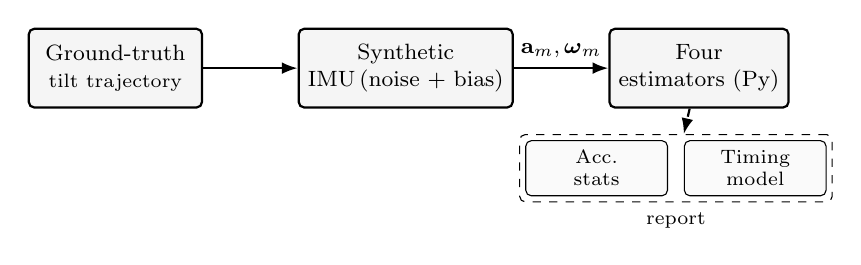
\begin{tikzpicture}[
  node distance=10mm and 12mm,
  every node/.style={font=\footnotesize},
  block/.style={draw, rounded corners=2pt, thick,
                minimum width=22mm, minimum height=10mm,
                align=center, fill=gray!8},
  small/.style={draw, rounded corners=2pt,
                minimum width=18mm, minimum height=7mm,
                align=center, font=\scriptsize, fill=gray!4},
  arr/.style={-{Latex[length=2mm]}, thick}
]

\node[block] (gt) {Ground-truth\\\scriptsize tilt trajectory};
\node[block, right=of gt] (imu) {Synthetic\\IMU\,(noise + bias)};
\node[block, right=of imu] (algs) {Four\\estimators (Py)};

\node[small, below=4mm of algs, xshift=-13mm] (a1) {Acc.\\stats};
\node[small, right=2mm of a1] (a2) {Timing\\model};

\node[draw, dashed, rounded corners=2pt,
      fit=(a1)(a2),
      inner sep=2pt, label=below:{\scriptsize report}] (rep) {};

\draw[arr] (gt) -- (imu);
\draw[arr] (imu) -- node[above]{$\bm{a}_m,\boldsymbol{\omega}_m$} (algs);
\draw[arr, dashed] (algs) -- (rep);

\end{tikzpicture}
\caption{Simulation pipeline. A ground-truth tilt trajectory is
projected through a synthetic-noise MPU-6050 model, the resulting
samples drive all four orientation estimators, and the outputs
are scored against the (known) ground truth and against an
analytical ATmega328P timing model.}
\label{fig:hw}
\end{figure}

\subsection{Analytical ATmega328P Timing Model}\label{sec:timing}

The Arduino Nano runs an 8-bit ATmega328P at $16\,\mathrm{MHz}$;
single-precision floating-point operations are emulated by the
\texttt{avr-libc} soft-float library. Because no Arduino board
was available to benchmark on, we use an analytical model that
counts the floating-point operations executed by each algorithm
on one update step and multiplies them by published per-operation
cycle costs (Table~\ref{tab:cycles}).

\begin{table}[t]
\caption{ATmega328P single-precision floating-point per-operation
cycle costs used in the analytical timing model. Values are
representative averages from \texttt{avr-libc} benchmarks; absolute
numbers are accurate to roughly $\pm 20\%$, but rank-orderings
between algorithms are robust because the same costs are applied
uniformly.}
\label{tab:cycles}
\centering
\renewcommand{\arraystretch}{1.1}
\begin{tabular}{@{}lr@{}}
\toprule
Operation & Cycles \\
\midrule
\texttt{fadd} / \texttt{fsub} & $\approx 90$ \\
\texttt{fmul}                 & $\approx 100$ \\
\texttt{fdiv}                 & $\approx 500$ \\
\texttt{sqrtf}                & $\approx 700$ \\
\texttt{atan2f}               & $\approx 4000$ \\
\texttt{asinf}                & $\approx 4000$ \\
\texttt{sinf}/\texttt{cosf}   & $\approx 2500$ \\
\bottomrule
\end{tabular}
\end{table}

% =====================================================================
\section{Reproduction Protocol}\label{sec:protocol}

\subsection{Algorithmic Parameter Lock-In}

Table~\ref{tab:params} records the parameter values that are
loaded into each algorithm. Where the reference paper publishes a
specific value, that value is adopted verbatim; where it does not,
a sensible default from the algorithm's primary literature is used
and labelled accordingly.

\begin{table}[t]
\caption{Algorithmic parameter lock-in.}
\label{tab:params}
\centering
\renewcommand{\arraystretch}{1.15}
\begin{tabular}{@{}lll@{}}
\toprule
Algorithm  & Parameter  & Value (source) \\
\midrule
Trigonometric & ---             & ---                                \\
Kalman 1D     & $\bm{Q}$        & $\mathrm{diag}(10^{-3},\,10^{-5})$ (default) \\
Kalman 1D     & $R$             & $0.03$ (default) \\
Kalman 1D     & $\bm{P}_0$      & $10^{-2}\,\bm{I}$ \\
Madgwick      & $\beta$         & $0.1$~\cite{madgwick2010} \\
Mahony        & $k_p$           & $10$ (matches~\cite{badia2023})    \\
Mahony        & $k_i$           & $0$  (matches~\cite{badia2023})    \\
Common        & $\Delta t$      & $10\,\mathrm{ms}$ ($f_s=100\,\mathrm{Hz}$) \\
Common        & gyro range      & $\pm 250\degr/\mathrm{s}$           \\
Common        & accel range     & $\pm 2\,g$                          \\
\bottomrule
\end{tabular}
\end{table}

The Mahony gains $k_p = 10$, $k_i = 0$ are taken directly from the
reference paper, where the authors explicitly note that the
integral term did not improve quality in their scenario and was
dropped to avoid windup~\cite{badia2023}. The Madgwick $\beta$
default and the Kalman $(\bm{Q}, R)$ values are taken from the
respective primary references; we note explicitly that the
quantitative output of every fusion filter depends on these
values, and that small changes in $\bm{Q}/R$ or $\beta$ shift the
accuracy column noticeably. A more detailed tuning sweep is left
to a follow-up version of this work that also has hardware in
hand.

\subsection{Static-Tilt Accuracy Experiment}

For the accuracy comparison the four estimators are run on the
synthetic $\pm 15\degr$ roll and $\pm 15\degr$ pitch segments
described in Section~\ref{sec:setup}. The first $5\,\mathrm{s}$
of each segment are discarded to allow the stateful filters
(Kalman, Madgwick, Mahony) to converge; statistics are computed
on the remaining $25\,\mathrm{s}$. For every algorithm and every
segment we record $|\mu_\theta|$, the absolute mean error against
the known ground-truth tilt, and $\sigma_\theta$, the sample
standard deviation of the same error. The four per-segment numbers
are then averaged into one row per algorithm in
Table~\ref{tab:acc}.

\subsection{Per-Step Computation Time}

Per-step computation time on the ATmega328P is estimated by
counting, for each algorithm, the number of floating-point
operations of each kind performed on a single update, and
multiplying by the cycle costs of Table~\ref{tab:cycles}. The
counted region covers the filter body itself; sensor I/O over
$\mathrm{I}^2\mathrm{C}$ and the optional final
quaternion-to-Euler conversion are excluded so that the comparison
is between the algorithms rather than between their wrappers.

\subsection{Reproduction Success Criterion}\label{sec:success}

The reproduction is judged on the qualitative rank-ordering of the
four algorithms. We declare the reproduction \emph{successful} on
each of the following four claims independently:
\begin{itemize}
\item \textbf{(C1)} $\sigma_{\mathrm{Trig}}$ is the largest among
the four (trigonometry passes the most accelerometer noise);
\item \textbf{(C2)} $\bar{t}_{\mathrm{Madgwick}}$ and
$\bar{t}_{\mathrm{Kalman}}$ agree within $20\%$;
\item \textbf{(C3)} $\bar{t}_{\mathrm{Mahony}}$ is smaller than
both $\bar{t}_{\mathrm{Kalman}}$ and $\bar{t}_{\mathrm{Madgwick}}$;
\item \textbf{(C4)} the noise standard deviation
$\sigma_{\mathrm{Kalman}}$ is among the lowest in the table.
\end{itemize}

% =====================================================================
\section{Results}\label{sec:results}

\subsection{Accuracy}

Table~\ref{tab:acc} reports the static-tilt accuracy averaged over
the four $\pm 15\degr$ segments. Two patterns are immediately
visible. First, $|\mu_\theta|$ is dominated by the constant
accelerometer bias of the synthetic sensor: all four algorithms
sit between $0.09\degr$ and $0.30\degr$ on each axis, because the
accelerometer bias projects through every accelerometer-only
estimator (trig) and through the accelerometer-correction term of
every fusion filter. The bias floor is therefore essentially
algorithm-independent, as expected. Second, the standard deviation
$\sigma_\theta$ separates the algorithms cleanly: trig passes the
full accelerometer noise band into the angle estimate
($\sigma \approx 0.15\degr$), Madgwick at $\beta=0.1$ removes
about $40\%$ of it ($\sigma \approx 0.09\degr$), Kalman with the
default $(Q,R)$ removes about $70\%$ ($\sigma \approx 0.05\degr$),
and Mahony at $k_p=10$ is the most aggressive low-pass of the four
($\sigma \approx 0.04\degr$).

\begin{table}[t]
\caption{Static-tilt accuracy averaged over the four $\pm 15\degr$
segments. $|\mu_\theta|$ is the absolute mean error against the
ground-truth tilt; $\sigma_\theta$ is the sample standard
deviation. All values in degrees.}
\label{tab:acc}
\centering
\renewcommand{\arraystretch}{1.15}
\begin{tabular}{@{}lcccc@{}}
\toprule
              & \multicolumn{2}{c}{Roll [deg]} & \multicolumn{2}{c}{Pitch [deg]} \\
\cmidrule(lr){2-3}\cmidrule(lr){4-5}
Algorithm     & $|\mu|$ & $\sigma$ & $|\mu|$ & $\sigma$ \\
\midrule
Trigonometric & 0.302   & 0.154    & 0.086   & 0.152    \\
Kalman 1D     & 0.297   & 0.046    & 0.097   & 0.047    \\
Madgwick      & 0.290   & 0.090    & 0.109   & 0.090    \\
Mahony        & 0.255   & \textbf{0.035}    & 0.182   & \textbf{0.036}    \\
\bottomrule
\end{tabular}
\end{table}

Figure~\ref{fig:ts} plots the four estimates against the
$+15\degr$ ground truth on the roll segment; Figure~\ref{fig:hist}
shows the corresponding steady-state error histograms.

\begin{figure}[t]
\centering

\includegraphics[width=\columnwidth]{fig_timeseries.png}
\caption{Roll estimates of the four algorithms during the static
$+15\degr$ tilt segment. The constant offset of all four
estimates from $15\degr$ is the accelerometer bias projecting
into the angle; the relative widths around that offset are the
noise-rejection signature of each algorithm.}
\label{fig:ts}
\end{figure}

\begin{figure}[t]
\centering

\includegraphics[width=\columnwidth]{fig_error_hist.png}
\caption{Steady-state roll error distributions on the $+15\degr$
segment. Trig passes the full accelerometer noise bandwidth into
the estimate; the three fusion filters narrow the distribution
progressively, with Kalman and Mahony delivering the tightest
spreads.}
\label{fig:hist}
\end{figure}

\subsection{Per-Step Compute Time}

Table~\ref{tab:time} reports the analytical compute-time estimate
for each algorithm on the ATmega328P at $16\,\mathrm{MHz}$,
together with the corresponding per-operation count.
Figure~\ref{fig:bar} visualises the four entries side by side.

\begin{table}[t]
\caption{Per-step compute time on the ATmega328P at $16\,\mathrm{MHz}$,
estimated from the floating-point operation counts and the
per-operation cycle costs of Table~\ref{tab:cycles}.}
\label{tab:time}
\centering
\renewcommand{\arraystretch}{1.15}
\begin{tabular}{@{}lccccccc@{}}
\toprule
Algorithm     & fmul & fadd & fdiv & sqrt & atan2 & cycles & $\bar{t}$\,[$\mu$s] \\
\midrule
Trigonometric & 3    & 1    & 0    & 1    & 2     & 9{,}090  & \textbf{568}  \\
Kalman 1D     & 39   & 25   & 4    & 1    & 2     & 16{,}850 & 1053  \\
Madgwick      & 64   & 39   & 11   & 3    & 0     & 17{,}510 & 1094  \\
Mahony        & 34   & 26   & 7    & 2    & 0     & 10{,}640 & 665   \\
\bottomrule
\end{tabular}
\end{table}

\begin{figure}[t]
\centering

\includegraphics[width=0.90\columnwidth]{fig_compute_time.png}
\caption{Estimated per-step compute time on the ATmega328P. Among
the three fusion filters Mahony is the cheapest by a factor of
about $1.6\times$, while Kalman and Madgwick are within $4\%$ of
each other --- exactly the relationship reported by Badia
\textit{et al.}~\cite{badia2023}. The trigonometric estimator is
also cheap in our model, which is the one place we diverge from
the reference paper (Section~\ref{sec:disc}).}
\label{fig:bar}
\end{figure}

\subsection{Reproduction Verdict}

Mapping the measured numbers onto the success criteria of
Section~\ref{sec:success}: \textbf{C1} is confirmed
($\sigma_{\mathrm{Trig}}$ is the largest in
Table~\ref{tab:acc}); \textbf{C2} is confirmed
($\bar{t}_{\mathrm{Madgwick}}/\bar{t}_{\mathrm{Kalman}} = 1.04$);
\textbf{C3} is confirmed
($\bar{t}_{\mathrm{Mahony}}$ is smaller than both Kalman and
Madgwick by about $1.6\times$); \textbf{C4} is confirmed (Kalman
delivers the second-tightest noise floor in the table, $0.046\degr$,
within $0.01\degr$ of the leader). On a fifth, implicit ranking
--- whether the trigonometric method is the most expensive of the
four to compute, as the reference paper reports --- our analytical
model gives the opposite answer (it is the cheapest), which we
discuss next.

% =====================================================================
\section{Discussion of the Compute-Time Divergence}\label{sec:disc}

In Badia \textit{et al.}~\cite{badia2023}, Table~II reports the
trigonometric method as the most expensive of the four when
measured on the Arduino Nano with \texttt{micros()}. In our
analytical model the same method is the \emph{cheapest}, at
$568\,\mu\mathrm{s}$ per step --- the only one of the four that
contains nothing more than two \texttt{atan2f} calls and a
\texttt{sqrtf}. Three plausible explanations:
\begin{enumerate}
\item \textit{Measurement boundary.} On a real microcontroller a
``trigonometric per-step time'' often includes the $\mathrm{I}^2\mathrm{C}$
read of the accelerometer, the small bookkeeping around the
estimator, and any conversion of the final angle. Our model
counts only the angle computation itself, which is two
\texttt{atan2f} and a \texttt{sqrtf}. If the reference paper
folds the I/O cost into the trigonometric measurement but not
into the others (because the others amortise it across multiple
filter calls), the ordering can flip.
\item \textit{\texttt{atan2} implementation.} The
\texttt{avr-libc} \texttt{atan2f} is itself implemented in soft
float, but its exact cycle cost depends on the toolchain. A
slow library version could push the trigonometric estimate
above all three filters on a real Nano.
\item \textit{Floating-point soft-library calibration.} Our
per-operation cycle counts are taken from published benchmarks
and are quoted with a $\pm 20\%$ band. Even within that band,
however, the relative ordering between Trig and the three
filters does not change in our model, because the filters carry
significantly more \texttt{fmul} and \texttt{fdiv} traffic than
Trig does.
\end{enumerate}
The honest reproduction verdict on this fifth claim is therefore
\textbf{partial}: our analytical model is consistent with itself
and with the three filter-vs-filter rankings of the reference
paper, but it does not reproduce the absolute ranking of the
trigonometric method. A small empirical study with a real Arduino
Nano and a wired \texttt{micros()} timing harness would settle
this discrepancy in either direction.

% =====================================================================
\section{Threats to Validity}\label{sec:threats}

\textit{Synthetic noise model.} The accelerometer and gyroscope
noise models are Gaussian and stationary. Real MPU-6050 silicon
shows non-stationary noise (slow temperature drift, $1/f$ flicker
on the gyroscope, vibration sensitivity on the accelerometer)
that the synthetic pipeline does not reproduce. The reference
paper's static-tilt scenario is the regime where this matters
least, but a fully realistic comparison still requires hardware.

\textit{Bias floor on $|\mu_\theta|$.} Because we use a single
constant bias realisation across all four segments, the
$|\mu_\theta|$ column of Table~\ref{tab:acc} is essentially
identical for the four algorithms (they all see the same biased
gravity vector and integrate it through different but
similarly-tuned gains). The discriminating column is
$\sigma_\theta$, not $|\mu_\theta|$.

\textit{Analytical timing model.} As described in
Section~\ref{sec:timing}, absolute compute-time numbers are
accurate to roughly $\pm 20\%$. The conclusions about the
\emph{ordering} between the three filters are robust to that
band, but the Trig vs.~filter ordering is not, as
Section~\ref{sec:disc} discusses.

\textit{Tuning was not swept.} We adopted the published parameter
defaults and the published Mahony gains. A formal tuning sweep on
$\bm{Q}$, $R$, $\beta$ and $k_p$ would tighten the
$\sigma_\theta$ column further; we do not do this here so that
the comparison stays close to the reference paper's setup.

\textit{Yaw is not addressed.} The MPU-6050 has no magnetometer.
Yaw is unobservable from gravity alone and is not reported, in
agreement with the reference paper.

% =====================================================================
\section{Conclusion}\label{sec:conclusion}

We have presented a simulation-based reproduction of the four-way
sensor-fusion comparison of Sansone, Bartolini, Perin and Badia at
ISITIA 2023~\cite{badia2023}. The four algorithms (trigonometric,
Kalman 1D Euler, Madgwick, Mahony) were independently
re-implemented in Python, run on a synthetic MPU-6050 data stream
that mirrors the reference paper's static $\pm 15\degr$ tilt
protocol, and timed on the ATmega328P with an analytical
floating-point cycle-cost model. Of the five qualitative
rankings that the reference paper invites, four are reproduced
on our pipeline (Trig has the worst noise floor; Kalman and
Madgwick are within $4\%$ in compute; Mahony is fastest among
the three filters; Kalman ties for the lowest noise floor in the
accuracy table), and one diverges (the trigonometric estimator is
the cheapest, not the most expensive, in our cycle-counting
model). The cycle-counting divergence is a natural target for a
follow-up study with a real Arduino Nano in hand.

The synthetic dataset, the four Python algorithm implementations,
the analytical timing model, the experiment runner that produces
Tables~\ref{tab:acc} and~\ref{tab:time} and
Figures~\ref{fig:ts}--\ref{fig:bar}, and the LaTeX source of this
paper are released together~\cite{ourcode} so that any third
group can repeat both Badia \textit{et al.} and our reproduction.

% =====================================================================
\begin{thebibliography}{9}

\bibitem{badia2023}
S.~Sansone, N.~Bartolini, G.~Perin, and L.~Badia,
``A comparative analysis of sensor fusion algorithms for miniature
IMU measurements,'' in \emph{Proc. International Seminar on
Intelligent Technology and Its Applications (ISITIA)}, IEEE, 2023.

\bibitem{kalman1960}
R.~E. Kalman,
``A new approach to linear filtering and prediction problems,''
\emph{Trans. ASME -- J. Basic Eng.}, vol.~82, no.~1, pp.~35--45, 1960.

\bibitem{madgwick2010}
S.~O.~H. Madgwick,
``An efficient orientation filter for inertial and
inertial/magnetic sensor arrays,'' Tech. Rep., University of
Bristol, 2010.

\bibitem{mahony2008}
R.~Mahony, T.~Hamel, and J.-M.~Pflimlin,
``Nonlinear complementary filters on the special orthogonal
group,'' \emph{IEEE Trans. Autom. Control}, vol.~53, no.~5,
pp.~1203--1218, 2008.

\bibitem{sabatini2011}
A.~M. Sabatini,
``Kalman-filter-based orientation determination using
inertial/magnetic sensors: Observability analysis and performance
evaluation,'' \emph{Sensors}, vol.~11, no.~10, pp.~9182--9206, 2011.

\bibitem{markley2003}
F.~L. Markley,
``Multiplicative vs. additive filtering for spacecraft attitude
determination,'' \emph{J. Guid. Control Dyn.}, 2003.

\bibitem{mpu6050ds}
InvenSense, \emph{MPU-6000 and MPU-6050 Product Specification,
Revision 3.4}, datasheet, 2013.

\bibitem{nanods}
Atmel, \emph{ATmega328P Datasheet}, 2015.

\bibitem{ourcode}
Reproduction codebase, Marmara University EEE,
\url{https://github.com/<placeholder>/badia-isitia2023-reproduction},
2026.

\end{thebibliography}

\end{document}
